\definecolor{yaml-bg}{HTML}{001B33}
\definecolor{yaml-prop}{HTML}{FF9D00}
\definecolor{yaml-str}{HTML}{3AD906}
\definecolor{yaml-num}{HTML}{FF0044}
\definecolor{tex-kw}{HTML}{F00000}
\definecolor{tex-env}{HTML}{5423D0}
\definecolor{tex-math}{HTML}{00A000}

% docker fill
\uncover<1->{%
  \fill[pattern=north east lines, pattern color=tu05light, rounded corners] (1.2,1.8) rectangle (6.6,-2.6)
    node[above left, anchor=south east, black!80] {\footnotesize Docker};
}

% meta-config
\uncover<2->{%
  \begin{scope}[scale=.78, transform shape, local bounding box=meta]
    \node[draw=gray, semithick, rectangle, fill=yaml-bg, text width=2cm, rounded corners, font=\ttfamily] at (0,0) {%
      \setlength{\baselineskip}{8pt}%
      \textcolor{yaml-prop}{\bfseries a\_1:} \textcolor{yaml-num}{1.0}\\[2pt]
      \textcolor{yaml-prop}{\bfseries dataset:}\\[1pt]
      \textcolor{white}{~~-} \textcolor{yaml-str}{fact}\\
      \textcolor{white}{~~-} \textcolor{yaml-str}{magic}
      \par % applies baselineskip to all lines
    };
  \end{scope}
  \node[below = 4mm, font=\small, align=center, text width=3cm] (metalab) at (meta.south) {Meta-Config\\[-2pt]\scriptsize(YAML)};
}

% job configs
\uncover<1->{%
  \begin{scope}[scale=.75, transform shape, shift={(3.25,-.1)}, local bounding box=jobs]
    \node[draw=gray, semithick, rectangle, fill=yaml-bg, text width=2.2cm, rounded corners, font=\ttfamily] at (.2,.2) {%
      \setlength{\baselineskip}{8pt}%
      \textcolor{yaml-prop}{\bfseries a\_1:} \textcolor{yaml-num}{1.0}\\[2pt]
      \textcolor{yaml-prop}{\bfseries data:} \textcolor{yaml-str}{magic}
      \par % applies baselineskip to all lines
    };
    \node[draw=gray, semithick, rectangle, fill=yaml-bg, text width=2.2cm, rounded corners, font=\ttfamily] at (0,0) {%
      \setlength{\baselineskip}{8pt}%
      \textcolor{yaml-prop}{\bfseries a\_1:} \textcolor{yaml-num}{1.0}\\[2pt]
      \textcolor{yaml-prop}{\bfseries data:} \textcolor{yaml-str}{fact}
      \par % applies baselineskip to all lines
    };
  \end{scope}
  \node[below, font=\small, align=center, text width=3cm] (joblab) at (jobs.south|-metalab.north) {Job Configs\\[-2pt]\scriptsize(YAML)};
}

% spectra
\uncover<1->{%
  \begin{scope}[scale=.85, transform shape, shift={(5.25,-.7)}, local bounding box=analysis]
    \begin{scope}[anchor=north east, shift={(.18,.18)}]
      % 
% This file was generated with Res.smearing_histogram("res/spectra/comparison_magic_uniform.csv"res/metrics/comparison_magic_uniform.csv")
% 
% git commit = c084a7e45bb1f3afd5999b1c80a6c3f4be207858
% git origin = git@bitbucket.org:mbunse/mt-exp.git
% uncommited changes = false
% 
\tikzstyle{every node} = [font=\small]

\begin{axis}[
  ylabel = {},
  xmin = {1.599999999999},
  xmax = {4.4000000000010004},
  xlabel = {},
  histogram axis,
  ymode = log,
  log origin y=infty,
  scale = .25,
  yticklabels = \empty,
  xticklabels = \empty,
  ylabel style = {rotate = 270, at = {(-.025,.5)}},
  xlabel style = {at = {(.5,-.025)}}
]
%   width = .75*\axisdefaultwidth,
%   height = .675*\axisdefaultheight,

% \addplot+[
%   histogram plot,
%   black,
%   thin,
%   name path = truth,
%   dash pattern={on 2.25pt off 0.75pt}
% ]
% coordinates {
%   (1.599999999999, 0.0)
%   (1.6, 0.06451926499999999)
%   (1.8333333333333333, 0.1221511)
%   (2.066666666666667, 0.1482697)
%   (2.3, 0.1439983)
%   (2.533333333333333, 0.1244045)
%   (2.7666666666666666, 0.10419795000000001)
%   (3.0, 0.08582171499999999)
%   (3.2333333333333334, 0.06412323500000001)
%   (3.466666666666667, 0.050539829999999994)
%   (3.7, 0.037032365)
%   (3.933333333333333, 0.027978120000000002)
%   (4.166666666666667, 0.026964024999999996)
%   (4.4, 0.026964024999999996)
%   (4.4000000000010004, 0.0)
% };
% \addlegendentry{$\mathbf{f}$}

\addplot+[
  histogram plot,
  tu02,
  very  thick,
  name path = estimate
]
coordinates {
  (1.599999999999, 0.0)
  (1.6, 0.07563379)
  (1.8333333333333333, 0.11441804999999998)
  (2.066666666666667, 0.14546300000000004)
  (2.3, 0.14178325)
  (2.533333333333333, 0.12264900000000004)
  (2.7666666666666666, 0.10740475000000001)
  (3.0, 0.086949075)
  (3.2333333333333334, 0.064010205)
  (3.466666666666667, 0.048701285000000004)
  (3.7, 0.03753382999999999)
  (3.933333333333333, 0.029620479999999998)
  (4.166666666666667, 0.025833409999999994)
  (4.4, 0.025833409999999994)
  (4.4000000000010004, 0.0)
};
% \addlegendentry{$\hat{\mathbf{f}}_\text{$\text{\sc Dsea}^+$}$}

% \addplot[draw=none, fill=tu01, fill opacity=0.33] fill between[of = truth and estimate];

% \legend{} % omit legend

\end{axis}


    \end{scope}
    \begin{scope}[anchor=north east, shift={(0,0)}]
      % 
% This file was generated with Res.smearing_histogram("res/spectra/comparison_magic_uniform.csv"res/metrics/comparison_magic_uniform.csv")
% 
% git commit = c084a7e45bb1f3afd5999b1c80a6c3f4be207858
% git origin = git@bitbucket.org:mbunse/mt-exp.git
% uncommited changes = false
% 
\tikzstyle{every node} = [font=\small]

\begin{axis}[
  ylabel = {$f$},
  xmin = {1.599999999999},
  xmax = {4.4000000000010004},
  xlabel = {energy},
  histogram axis,
  ymode = log,
  log origin y=infty,
  scale = .25,
  yticklabels = \empty,
  xticklabels = \empty,
  ylabel style = {rotate = 270, at = {(-.025,.5)}},
  xlabel style = {at = {(.5,-.025)}}
]
%   width = .75*\axisdefaultwidth,
%   height = .675*\axisdefaultheight,

% \addplot+[
%   histogram plot,
%   black,
%   thin,
%   name path = truth,
%   dash pattern={on 2.25pt off 0.75pt}
% ]
% coordinates {
%   (1.599999999999, 0.0)
%   (1.6, 0.06451926499999999)
%   (1.8333333333333333, 0.1221511)
%   (2.066666666666667, 0.1482697)
%   (2.3, 0.1439983)
%   (2.533333333333333, 0.1244045)
%   (2.7666666666666666, 0.10419795000000001)
%   (3.0, 0.08582171499999999)
%   (3.2333333333333334, 0.06412323500000001)
%   (3.466666666666667, 0.050539829999999994)
%   (3.7, 0.037032365)
%   (3.933333333333333, 0.027978120000000002)
%   (4.166666666666667, 0.026964024999999996)
%   (4.4, 0.026964024999999996)
%   (4.4000000000010004, 0.0)
% };
% \addlegendentry{$\mathbf{f}$}

\addplot+[
  histogram plot,
  tu01,
  very  thick,
  name path = estimate
]
coordinates {
  (1.599999999999, 0.0)
  (1.6, 0.07563379)
  (1.8333333333333333, 0.11441804999999998)
  (2.066666666666667, 0.14546300000000004)
  (2.3, 0.14178325)
  (2.533333333333333, 0.12264900000000004)
  (2.7666666666666666, 0.10740475000000001)
  (3.0, 0.086949075)
  (3.2333333333333334, 0.064010205)
  (3.466666666666667, 0.048701285000000004)
  (3.7, 0.03753382999999999)
  (3.933333333333333, 0.029620479999999998)
  (4.166666666666667, 0.025833409999999994)
  (4.4, 0.025833409999999994)
  (4.4000000000010004, 0.0)
};
% \addlegendentry{$\hat{\mathbf{f}}_\text{$\text{\sc Dsea}^+$}$}

% \addplot[draw=none, fill=tu01, fill opacity=0.33] fill between[of = truth and estimate];

% \legend{} % omit legend

\end{axis}


    \end{scope}
  \end{scope}
  \node[below, font=\small, align=center, text width=3cm] at (analysis.south|-metalab.north) {Analysis Results\\[-2pt]\scriptsize(CSV)};
}

% metrics
\uncover<3->{%
  \begin{scope}[scale=.75, transform shape, shift={(10.25,-.1)}, local bounding box=metrics]
    \node at (0,0) {%
      \scriptsize
      \setlength{\tabcolsep}{4pt}
      \renewcommand{\arraystretch}{1.12}
      \begin{tabular}{c|c|c}
	{\bf data} & {\bf k} & {\bf EMD} \\
	\hline
	fact & 1 & 0.12 \\[-2pt]
	fact & 2 & 0.08 \\[-2pt]
	magic & 1 & 0.14 \\[-2pt]
	\vdots & \vdots & \vdots
      \end{tabular}
    };
  \end{scope}
  \node[below, font=\small, align=center, text width=3cm] at (metrics.south|-metalab.north) {Metrics\\[-2pt]\scriptsize(CSV)};
}

% tex code
\uncover<5->{%
  \begin{scope}[scale=.8, transform shape, shift={(12.75,-.2)}, local bounding box=plot]
    \node[text width=2.4cm, font=\ttfamily, fill=lightgray!66, rounded corners, inner sep=6pt] at (0,0) {%
      \scriptsize
      \setlength{\baselineskip}{-0pt}%
      \textcolor{tex-kw}{\textbackslash begin}\{\textcolor{tex-env}{axis}\}[\\
      ~~ylabel = \{\textcolor{tex-math}{\$f\$}\},\\
      ~~xmin = \{1.59\},\\
      ~~xmax = \{4.40\},\\[3pt]
      ~~\dots
      \par
    };
  \end{scope}
  \node[below, font=\small, align=center, text width=3cm] (plotlab) at (plot.south|-metalab.north) {Plot\\[-2pt]\scriptsize(TeX)};
  \node[below=3mm, rotate=-9, font=\small\bfseries, align=center, text width=3cm, tu01] at (plotlab.south) {versioning info\\embedded!};
}

% plots / paper
\uncover<6->{%
  \begin{scope}[shift={(12.65,-.06)}, local bounding box=paper]
    \node[inner sep=0pt] at (0,0) {%
      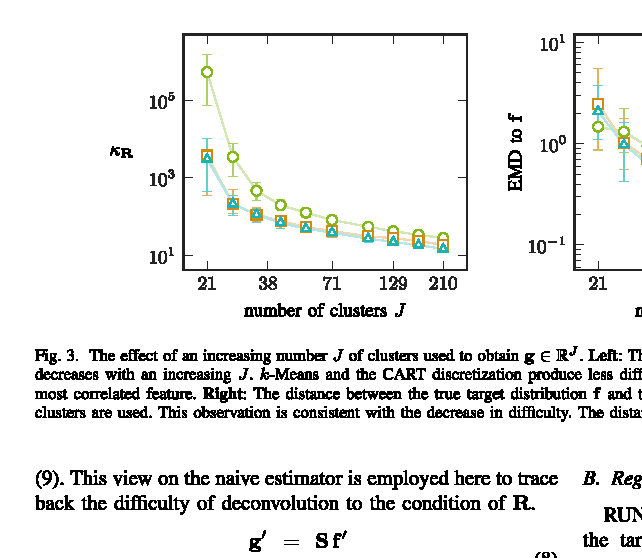
\includegraphics[scale=.16]{img/tex/embed}
    };
  \end{scope}
  \node[below, font=\small, align=center, text width=3cm] at (paper.south|-metalab.north) {Paper\\[-2pt]\scriptsize(PDF)};
}

% arrows
\uncover<2->{%
  \draw[thick] ($(meta.north)+(15pt,2pt)$) edge[->, bend left=50]
    node[pos=.45, above, font=\footnotesize] {split} ($(jobs.north)+(-15pt,2pt)$);
}
\uncover<1->{%
  \draw[thick] ($(jobs.north)+(15pt,2pt)$) edge[->, bend left=50]
    node[pos=.6, above, font=\footnotesize]  {run experiments} ($(analysis.north)+(-15pt,2pt)$);
}
\uncover<3->{%
  \draw[thick] ($(analysis.north)+(20pt,2pt)$) edge[->, bend left=50]
    node[pos=.5, above, font=\footnotesize]  {evaluate} ($(metrics.north)+(-10pt,2pt)$);
}
\uncover<5->{%
  \draw[thick] ($(metrics.north)+(15pt,2pt)$) edge[->, bend left=50]
    node[pos=.5, above, font=\footnotesize]  {aggregate} ($(plot.north)+(-20pt,2pt)$);
}
\uncover<6->{%
  \draw[thick] ($(plot.north)+(15pt,2pt)$) edge[->, bend left=50]
    node[pos=.5, above, font=\footnotesize]  {embed} ($(paper.north)+(-15pt,2pt)$);
}

% workflow
\uncover<4->{%
  \draw[<-, ultra thick] ($(jobs.south)+(0,-25mm)$) -- ($(jobs.south)+(0,-30mm)$)
    node[below=1mm, text width=4cm, align=center] (pushlab) {push code, data \& configs};
  \draw[->, ultra thick] ($(jobs.south)+(2.75,-25mm)$) -- ($(jobs.south)+(2.75,-30mm)$)
    node[below=1mm, text width=4cm, align=center] {pull\\results};
}